% ----------------------- Becoming a Gentoo Developer -------------------------
\section{Recruiting}

\subsection{Becoming a Gentoo Developer}
\begin{frame}{Getting your Gentoo Developer Badge}
Long process, requires time, patience and deep understanding of the Gentoo Organizational and Technical policies.
\\~\\
Required Steps
	\begin{itemize}
		\item Find a mentor!
		\item Ebuild Quiz
		\item End Quiz
		\item Series of interviews with a recruiter
		\item Practical Test
	\end{itemize}
\end{frame}
%------------------------------------------------------------------------------

% ----------------------- What you get as a Developer -------------------------
\begin{frame}{Why?}
Get +w access to our git, svn and gentoo-x86 cvs (a.k.a portage) trees
\\~\\
Also
	\begin{itemize}
		\item \$\{yournickname\}@gentoo.org email (cool huh?)
		\item Improve (or rather serve!) your beloved distro
		\item Experience
		\item Meet new people
		\item Epic flames that you wouldn't want to miss
	\end{itemize}
\end{frame}
%------------------------------------------------------------------------------

%----------------------- Improving Recruitment Process-------------------------
\subsection{Improving the Recruitment Process}
\begin{frame}{What can be done?}
As said, long (like really *really* long) process
\\~\\
Is there room for improvements?
	\begin{itemize}
		\item Improved webapp?
	 	\item Google Docs (either for quiz submission or real-time tests)?
	 	\item G+ Hangouts?
	 	\item Other? Ideas? Please tell me!
	\end{itemize}
\end{frame}
%------------------------------------------------------------------------------

% ----------------------- Recruitment Performance -------------------------
\subsection{How do we perform?}
\begin{frame}{Recruitment Statistics}
	\begin{center}
	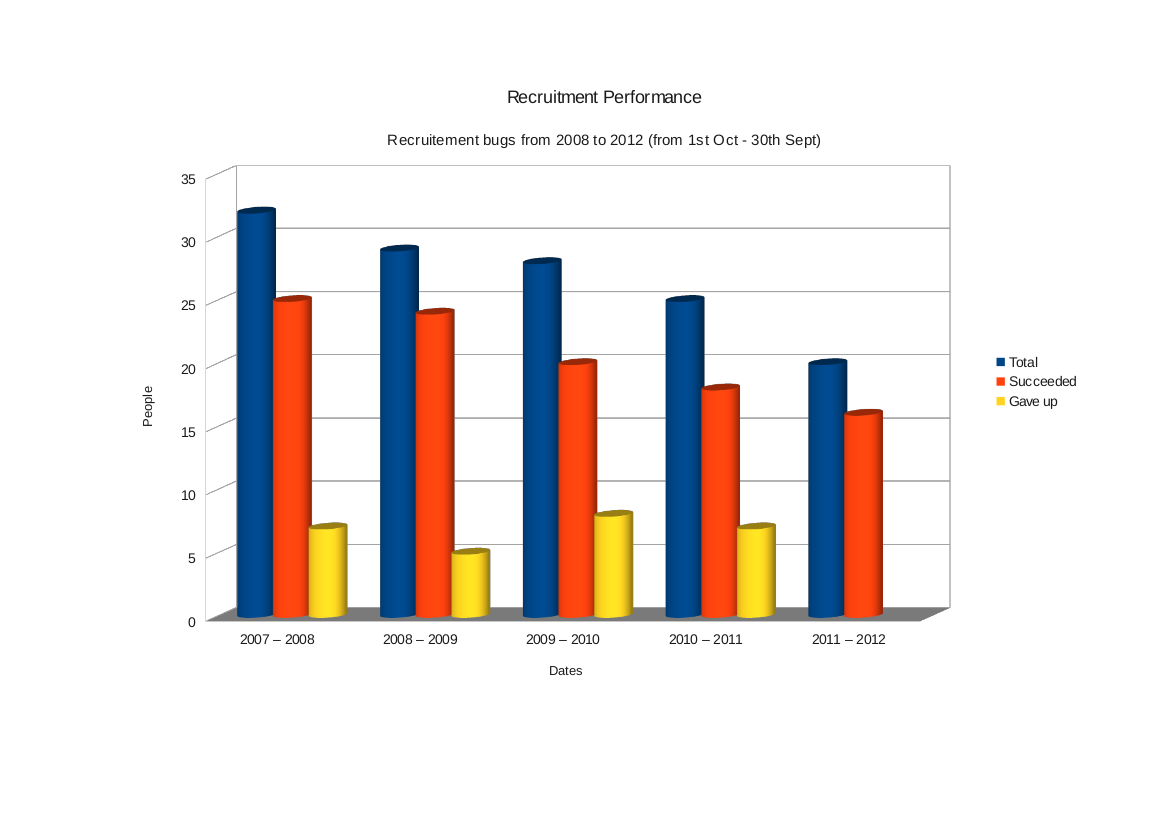
\includegraphics[scale=0.32]{recruitment_stats.png}
	\end{center}
\end{frame}
%------------------------------------------------------------------------------

%------------------------- Proxy Maintainers ----------------------------------
\subsection{Other ways to help us}
\begin{frame}{Proxy Maintainers}
	\begin{center}
	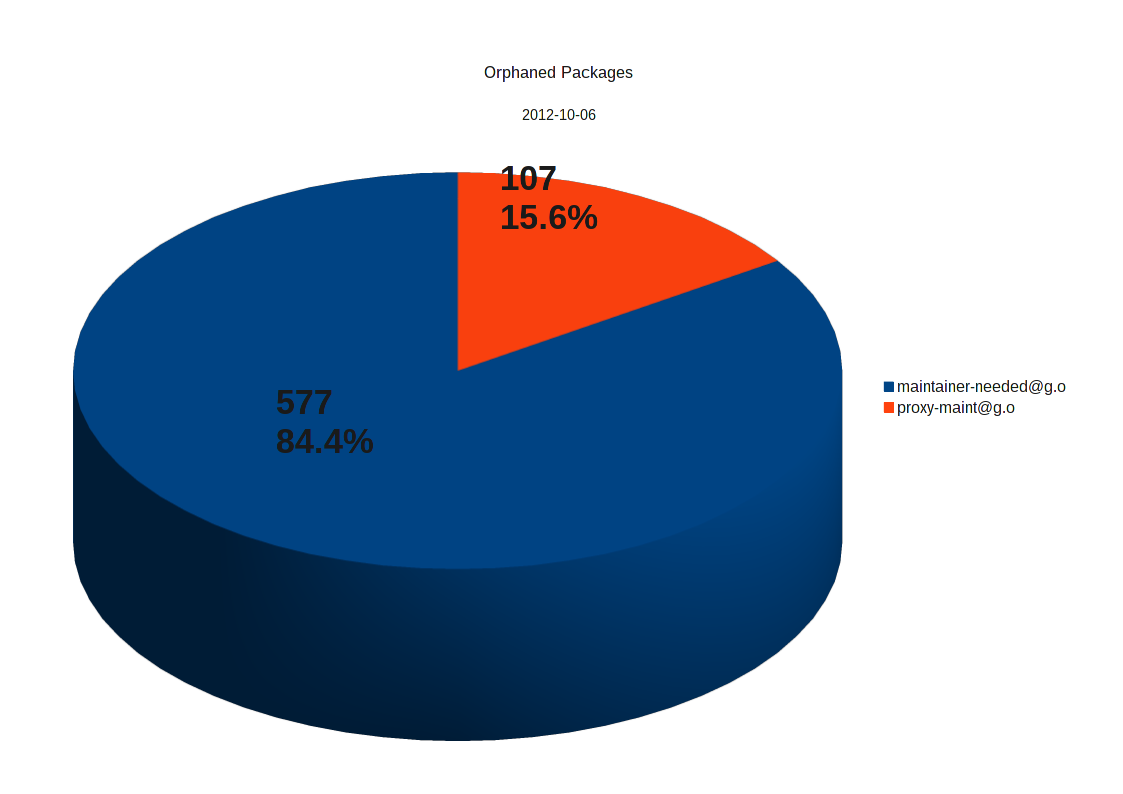
\includegraphics[scale=0.28]{orphaned_packages.png}
	\end{center}
\end{frame}
%------------------------------------------------------------------------------

%------------------------- AT/HT ----------------------------------
\begin{frame}{Arch / Herd Testers}
All we need is your CPU cycles (Ok and some RAM too)
	\begin{itemize}
	\item AT: Use your stable amd64/x86/\$\{arch\} box to help us stabilize more packages
	\item HT: Build, run, crash the testing packages for your favorite herd (kde, lxde, chromium etc.). Less work for ATs ;-)
	\end{itemize}
\end{frame}
%------------------------------------------------------------------------------

%---------------------- Help Needed -------------------------------------------
\subsection{We need help}
\begin{frame}{Where do we need help?}
	\begin{itemize}
		\item \href{http://www.gentoo.org/proj/en/devrel/staffing-needs/}{http://www.gentoo.org/proj/en/devrel/staffing-needs/}
		\item \href{http://www.gentoo.org/proj/en/qa/treecleaners/maintainer-needed.xml}{http://www.gentoo.org/proj/en/qa/treecleaners/maintainer-needed.xml}
		\item Search for long-standing open bugs, submit patches, then contact proxy-maint@gentoo.org
		\item We are always looking for new people even if you don't know what you want to do
	\end{itemize}
\begin{center}Contact us: recruiters@gentoo.org\end{center}
\end{frame}
%------------------------------------------------------------------------------
